\chapter{Introduction}\label{chapter:introduction}

Game theory is a field that makes use of mathematical tools and logic to model
and analyse situations of conflict, cooperation, and competition. One of the
most well-known examples of a strategic game is the Prisoner's Dilemma,
consisting of two players which can either cooperative or defect. A more
realistic version of the game is that of the Iterated Prisoner's Dilemma where
the two players play more than once in succession. The players remember the
previous actions taken and change their strategy accordingly.

The world is surrounded by situations of conflict, and understanding the
emergent outcome of interactions between two players can have a significant impact in
economical and political sciences.

In 1984 the ``The evolution of Cooperation'' was published by Robert Axelrod
introducing the usage of the Iterated Prisoner's Dilemma and computer modelling
in studying situations of conflict. Axelrod explored the optimal behaviour of
players in round robin tournaments using computer strategies. Many tournaments
have followed Axelrod's, and today the literature and various codebases
contain hundreds of strategies. The aim of all these strategies has been to capture
the best behaviour when playing the game.

This thesis aims to reinforce the understanding of optimal behaviour in the
Prisoner's Dilemma for a variety of environments. It summarises,
evaluates and builds upon previous literature. It does not only contribute to
the discussion of dominant behaviour but also provides new mathematical results
for the continued understanding of the questions raised throughout.

This introductory Chapter is set as follows:

\begin{itemize}
    \item section~\ref{section:introduction_prisoners_dilemma} introduces
    the Prisoner's Dilemma.
    \item section~\ref{section:introduction_brief_literature} covers a brief
    literature review.
    \item section~\ref{section:introduction_research_questions} formalises the research
    questions and sets out the structure of the thesis.
    \item section~\ref{section:introduction_software_development} presents the
    software development techniques used throughout the thesis.
\end{itemize}

\section{Prisoner's Dilemma}\label{section:introduction_prisoners_dilemma}

Game theory was formalised in 1944~\cite{VonNeumann1944} and is the study of
interactions as \textit{games}. A game is a model of interacting
decision makers referred to as \textit{players}. Each player has a set of
possible \textit{actions}, and the game captures the interactions of the players'
actions by allowing each player's \textit{payoffs} to be dependant on the actions
of all players. More precisely, as given in~\cite{Osborne2004}, the formal
definition of a game is as follows:

\begin{definition}
A \textbf{game} consists of
\begin{itemize}
    \item a set of players,
    \item for each player, a set of actions and
    \item for each player, payoff functions mapping the set of all actions to a numerical value.
\end{itemize}
\end{definition}

One of the most well known games is the Prisoner's Dilemma (PD) originally
described in~\cite{Flood1958}. The PD is a two player non-cooperative game which
illustrates aspects of political philosophy and morality; how selfishness will
lead to an `inefficiency' of the outcome even though selflessness can be
evolutionarily advantageous.

More specifically, in the PD each player has two actions, to either be selfless
and cooperate, denoted as ($C$), or to be selfish and defect, denoted as ($D$). Each
decision is made simultaneously and independently. The players' payoffs are
generally represented by Equation (\ref{eq:pd_definition}). Both players receive a reward
for mutual cooperation, \(R\), and a payoff \(P\) for mutual defection. A player
that defects while the other cooperates receives a payoff of \(T\), whereas the
cooperator receives \(S\).

\begin{equation}\label{eq:pd_definition}
    S_p =
    \begin{pmatrix}
        R & S  \\
        T & P
    \end{pmatrix}
    \quad
    S_q =
    \begin{pmatrix}
        R & T  \\
        S & P
    \end{pmatrix}
\end{equation}

It is assumed that two cooperating players do better than two defecting ones,
and thus, the payoff of two cooperating players is
larger than the payoff of two defecting players; \(R > P\). A player, however, has the
temptation to deviate, as that player will receive a higher payoff \(T\) than
that of mutual cooperation \(R\) whilst the cooperator's payoff \(S\) is smaller than
\(P\). In consequence, the payoffs are constrained by
Equation~(\ref{eq:constrain_one}).

\begin{equation}\label{eq:constrain_one}
    T > R > P > S
\end{equation}

A second constraint which ensures that a social dilemma arises, is that the sum
of the utilities to both players is best when they both cooperate,
Equation~(\ref{eq:constrain_two}).

\begin{equation}\label{eq:constrain_two}
    2R > T + S
\end{equation}

An equivalent representation of the PD is the \textit{donation game}. In the
donation game each player can cooperate by providing a benefit \(b\) to the
other player at a cost \(c\) with \(0 < c < d\). Thus, the players' payoffs for
the donation game are as given by Equation~(\ref{eq:the_pd_payoffs_with_cost}).

\begin{equation}\label{eq:the_pd_payoffs_with_cost}
    S_p =
    \begin{pmatrix}
        b - c & c\\
        b & 0
    \end{pmatrix}
    \quad
    S_q =
    \begin{pmatrix}
        b - c & b  \\
        c & 0
    \end{pmatrix}
\end{equation}

This thesis studies the PD as given by Equation~(\ref{eq:pd_definition}). There
are numerical experiments presented in the following Chapters. These have been
carried out using the payoff values of \(R = 3, P = 1, T = 5\) and \(S =
0\), which are the values most commonly used in the
literature~\cite{Adami2013, Axelrod1984,  Beaufils1988, Bendor1991, Donninger1986,
Franken2005, Knight2017, Harper2017, kendall2007iterated, Knight2018, Li2007,
A.Rogers2007Ctpw, Stewart2012}.

In non-cooperative games the players interact in order to achieve their best 
possible outcome. A \textit{best response strategy} is a strategy
that maximises the utility of a player given a known strategy of the other
player. A solution concept commonly used in game theory is the Nash equilibrium~\cite{Nash1951}
which is a pair of best response strategies at which neither of the players has
a reason to deviate.

In the PD due to constraint (\ref{eq:constrain_one}) it never benefits a player
to cooperate. A player that cooperates receives either a payoff of \(R\) or \(S\)
depending the action of the other player, whereas if a player defects they
receive either \(T\) or \(P\), and \(T > R\) and \(P > S\). Once both
players defect neither have a reason to change their decision. Thus, in the
PD mutual defection is a Nash equilibrium and defection is the
best response strategy.

The game can be studied in a manner where prior outcomes matter. The repeated
form of the game is called the Iterated Prisoner's Dilemma (IPD) and it differs
from the original concept of a PD because participants can learn about the
behavioural tendencies of their opponent. In the IPD defecting is no
longer necessarily the dominant action, and identifying a best response is not
always trivial.

\section{Brief history of the IPD}\label{section:introduction_brief_literature}

In the 1980's Robert Axelrod studied the best way of behaving in the IPD by
running a series of computer tournaments with two collections of
strategies~\cite{Axelrod1984}. These strategies were written/submitted by
researchers. Axelrod performed an evolutionary tournament~\cite{Axelrod1981} and
two round robin tournaments~\cite{Axelrod1980a, Axelrod1980b}. The strategy that
took over the population and won both tournaments was the strategy \TitForTat.
Axelrod's results demonstrated the robustness of the strategy in those
environments and subsequently the robustness of reciprocal behaviour. These
results, however, did not consider the success of the strategy in other
environments. This became more evident as further competitions and mathematical
formulations introduced new dominant strategies. A
brief summary of selected works and their dominant strategies are given by
Table~\ref{table:tournament_refs}.

\begin{table}[htbp]
    \centering
    \resizebox{\textwidth}{!}{
    \begin{tabular}{ccll}
        \toprule
        Year & Reference & Environment & Dominating Strategies\\
        \midrule
        1980 & \cite{Axelrod1980a} & Round robin tournament with 13 participants & \TitForTat \\
        1980 & \cite{Axelrod1980b} & Round robin tournament with a probabilistic ending and 13 participants & \TitForTat\\
        1984 & \cite{Axelrod1981}  & Ecological tournament with 64 participants & \TitForTat \\
        1987 & \cite{Beaufils1997} & Round robin \& ecological tournament with 12 participants & \Gradual \\
        1991 & \cite{Bendor1991}   & Round robin tournament with noise and 13 participants & \NiceandForgiving \\
        2005 & \cite{kendall2007iterated}  & Varied with 223 participants & Varying \\
        2012 & \cite{Stewart2012}  & Round robin tournament with 13 & Generous zero-determinants \\
        2016 & \cite{Knight2016}   & Round robin tournament with 130 participants & Heuristically trained strategies\\
        2017 & \cite{Harper2017}   & Round robin tournament with 200 participants & Heuristically trained strategies\\
        \bottomrule
    \end{tabular}}
    \caption{An overview of published works that introduced dominating IPD strategies in their
    respective environments. These strategies were either explicitly calculated,
    intelligently designed, or were developed through training methods.}
    \label{table:tournament_refs}
\end{table}

More details on these works will be presented in
Chapter~\ref{chapter:literature_review}, and following
Chapters~\ref{chapter:literature_review} and~\ref{chapter:bibliometric_study}
it will become evident that the literature on the IPD is rich, and new
strategies and competitions are being published every year.
The question, however, still remains the same: what is the best way to
play the game?

\section{Research questions \& Thesis structure}\label{section:introduction_research_questions}

This thesis contains eight Chapters, which together attempt to answer the research
question:

\begin{itemize}
    \centering
    \item[] What is the optimal behaviour an Iterated Prisoner's Dilemma strategy should
    adopt as a response to different environments?
\end{itemize}

Initially, Chapter~\ref{chapter:literature_review} provides a condensed
literature review which summarises the already established results of the
literature. Chapter~\ref{chapter:literature_review} separates the reviewed manuscripts
under different research topics identified manually. To complement the manual
separation of articles under research topics,
Chapter~\ref{chapter:bibliometric_study} automatically partitions \totalarticles IPD
articles using data mining, machine learning and natural language processing. The data set of \totalarticles articles' metadata has
been collected using a bespoke research software tool, which was written for this work but has since been used by others. The data set is further
analysed using network theoretic approaches to explore the behaviour of authors.

There are four Chapters to the thesis which explore optimal behaviour using original approaches. Namely,
Chapter~\ref{chapter:meta_tournaments} analyses a set of \numberofalltournaments computer
tournaments of distinct types and evaluates \numberofstrategies strategies'
performance. Chapter~\ref{chapter:memory_one} explores best response strategies
to environments of memory-one opponents and
Chapter~\ref{chapter:best_response_sequence} explores best response strategies
in the form of static sequences of moves to a collection of opponents. Finally
Chapter~\ref{chapter:lstm}, uses the data set of best response sequences
generated in Chapter~\ref{chapter:best_response_sequence} to train an IPD
strategy using a recurrent neural network.

The six Chapters of the thesis and their role is illustrated in
Figure~\ref{fig:structure_of_thesis}. An arrow between one Chapter and another
implies that the work described in one serves as motivation for the other.

\begin{figure}[!hbtp]
    \centering
    \includestandalone[width=\textwidth]{src/chapters/01/tex/thesis_structure}
    \caption{Structure of this thesis.}\label{fig:structure_of_thesis}
\end{figure}

A summary of each Chapter is given below:

\begin{itemize}
    \item Chapter~\ref{chapter:introduction} has contextualised the three main
    research questions of this thesis. Background of game theory and the
    PD has been given, and the structure
    of the remainder of the thesis has been outlined.
    \item Chapter~\ref{chapter:literature_review} provides a
    literature review for the PD and a manual classification of
    the reviewed papers under research topics. The manually identified research
    topics include evolutionary dynamics, intelligently designed strategies
    and structured strategies which have undergone training.
    \item Chapter~\ref{chapter:bibliometric_study} presents a bibliometric
    analysis of \totalarticles IPD articles. It uses natural language processing to
    identify five research topics, and a graph theoretic approach to quantify the
    collaborativeness of the field. The five identified topics are human subject
    research, biological studies, strategies, evolutionary dynamics on networks
    and modelling problems as a PD.
    \item Chapter~\ref{chapter:meta_tournaments} generates and analyses a set of
    \numberofalltournaments computer tournaments. It evaluates
    \numberofstrategies strategies, many of which are well known strategies from
    the literature. It presents the top performing strategies and analyses their
    salient features. The results show that there is not yet a single strategy
    that performs well in diverse IPD scenarios,
    nevertheless there are several properties that heavily influence the best
    performing strategies. These are: be nice, be provocable and generous, be a
    little envious, be clever, and adapt to the environment.
    \item Chapter~\ref{chapter:memory_one} explores best responses to a
    collection of memory-one strategies as a multidimensional non-linear
    optimisation problem. It presents a closed form algebraic expression for the
    utility of a memory-one strategy against a given set of opponents, a
    compact method of identifying its best response to that given set of
    opponents whilst having a theory of mind, and it introduces a well designed
    framework that allows the comparison of an optimal memory-one strategy and a
    more complex strategy which has a larger memory. The results add to the
    literature that has shown that extortionate play is not always optimal by
    showing that optimal play is often not extortionate.
    \item Chapter~\ref{chapter:best_response_sequence} explores the problem of
    IPD best responses in the form of sequences.
    It heuristically identifies the best response sequence against \numberofstrategiesbestsequences strategies,
    and generates a data set of 750 best response sequences of 205 turns.
    The Chapter mainly serves as a foundation for Chapter~\ref{chapter:lstm}
    but does present a novel heuristic and a study of its performance.
    \item Chapter~\ref{chapter:lstm} uses the data set of best response
    strategies obtained from Chapter~\ref{chapter:best_response_sequence} to
    train a type of recurrent neural network to predict best response sequences.
    The recurrent neural network used is the long short-term memory network
    (LSTM) which has gained a lot of attention in the machine learning
    literature but not in the IPD literature. A total of \lstmnetworks were
    trained which were then used to introduce \lstmstrategies distinct IPD
    strategies. It is demonstrated that a set of these strategies can win
    standard tournaments and the best LSTM performers on average rank at the top
    25\% of any standard tournament.
    \item Chapter~\ref{chapter:conclusion} summarises the work of the previous
    chapters, and indicates possible directions of future work, identifying
    further research questions that have arisen.
\end{itemize}

Chapters~\ref{chapter:meta_tournaments}-\ref{chapter:lstm} explore optimal
behaviour in the IPD. The disparity between the
approaches is their depth, as illustrated in Figure~\ref{fig:depth_structure}.
Chapter~\ref{chapter:meta_tournaments} explores optimal behaviour
by analysing a data set of tournaments and evaluating the performance of
pre-designed strategies. The exact opposite is done in
Chapter~\ref{chapter:memory_one} whereas for a given set of two
memory-one opponents a best response strategy is calculated explicitly.
Similarly, a best responses sequence against a given opponent is calculated in
Chapter~\ref{chapter:best_response_sequence}, but this is done using a heuristic
method. Finally, Chapter~\ref{chapter:lstm} uses a machine learning algorithm
to generate a optimal behaviour based on recurrent networks without any manual
input.

\begin{figure}[!hbtp]
    \centering
    \includestandalone[width=.9\textwidth]{src/chapters/01/tex/depth_structure}
    \caption{The depth of exploration whilst reporting on research question 1.}\label{fig:depth_structure}
\end{figure}

Most of Chapters of the thesis make use of parameters. There are instances that
the same symbol is used at different Chapters to denote different parameters
with different meanings. The parameters of each Chapter alongside a brief
exploration per Chapter is given in the
Appendix~\ref{appendix:parameters_per_chapter}.

\section{Software development \& Best practices}\label{section:introduction_software_development}

A survey conducted by the Software Sustainability Institute at 15 Russell Group
Universities showed that 92\% of the researchers questioned use software
intensively in their work, and 70\% said that ``It would not be practical to
conduct my work without software''~\cite{ssi_blog}. Similarly, the research of
this thesis heavily relies on software. As with all research there is an
obligation to ensuring the correctness and reproducibility of the results and the
software decisions throughout this thesis have been driven by these
requirements.

For the research of each Chapter (excluding Chapters~\ref{chapter:literature_review}
and~\ref{chapter:conclusion}) source code and analysis code have been developed.
All code is written in the an open source language Python, has been made public
via GitHub and has one of the most flexible and permissive licences, the MIT
licence. Essentially, the code developed for the thesis is available for inspection,
testing, and modification which enables and encourages
greater understanding of the underlying methodology, increases model confidence,
and provides an extendable framework which can be used by others.

Two themes arise as vital in research software development:
reproducibility and sustainability. To reassure the reproducibility and
sustainability of the software, and subsequently the research described in the
thesis, several methods of
\textit{best practice}~\cite{Aberdour2007, Benureau2018, Crick2014, Hong2015}
were considered and implemented during development. Namely:

\begin{itemize}
    \item Version control
    \item Virtual environments
    \item Automated testing
    \item Documentation
\end{itemize}

These will be discussed in the following subsections.

\subsection{Version control}

\textit{Version control}, is a system which records all files that make up a
project (down to the line) over time, tracking their development. It also
provides the ability to recall previous versions of files. This type of system
is essential for ensuring reproducibility of scientific research~\cite{Sandve2013,
Wilson2014}.

A good version control system has the following features as stated in~\cite{Ruparelia2010}:

\begin{itemize}
    \item Backup and restore: Files can be saved as they are edited and have the facility to
    jump to a previous version.
    \item Synchronisation: Source code files can be shared and users can update their
    codebase with the latest version.
    \item Undo changes: Changes made to the code can be undone by going back
    to a version that was committed in the past.
    \item Track changes: Messages are attacked to file changes in order to track the
    how and why the code evolved over time.
    \item Track ownership: File changes are tagged with the user's name who made
    the changes.
    \item Sandboxing: The ability to make temporary changes in an isolated area,
    called a sandbox, to test and try out code before it is checked in.
    \item Branching and merging: This is akin to a larger sandbox. Users can
    branch a copy of the code into a separate area and modify it in
    isolation (tracking changes separately). Later, the work can be merged back
    into the original codebase.
\end{itemize}

There are a number of popular tools for version control, these include Git~\cite{git},
Subversion~\cite{subversion}, and Mercurial~\cite{mercurial}. The version
control system chosen to carry out the software development here is Git.

There are several services that host Git servers online and allow users to work
with Git publicly. These services are essential for reproducibility as they make
not only the source code for the computer programmes available online but also
the history of its development. Such services are GitHub~\cite{github},
SourceForge~\cite{sourceforge}, GitLab~\cite{gitlab}, and BitBucket~\cite{bitbucket}.
GitHub is the chosen service for the thesis which integrates well with Git.

An important feature of GitHub is that it fosters collaboration between users.
It is a social service which allows users to comment and raise issues on each
other's repositories. Moreover, it encourages collaboration and code contributions
by other users through pull request features. An example of a pull request on
a GitHub repository is given by Figure~\ref{fig:pull_request_github}. In Figure~\ref{fig:pull_request_github}
it is shown how changes are tagged with a user and a short message describing
the alternations made to the codebase.

\begin{figure}[!htbp]
\begin{subfigure}{0.5\textwidth}
    \centering
    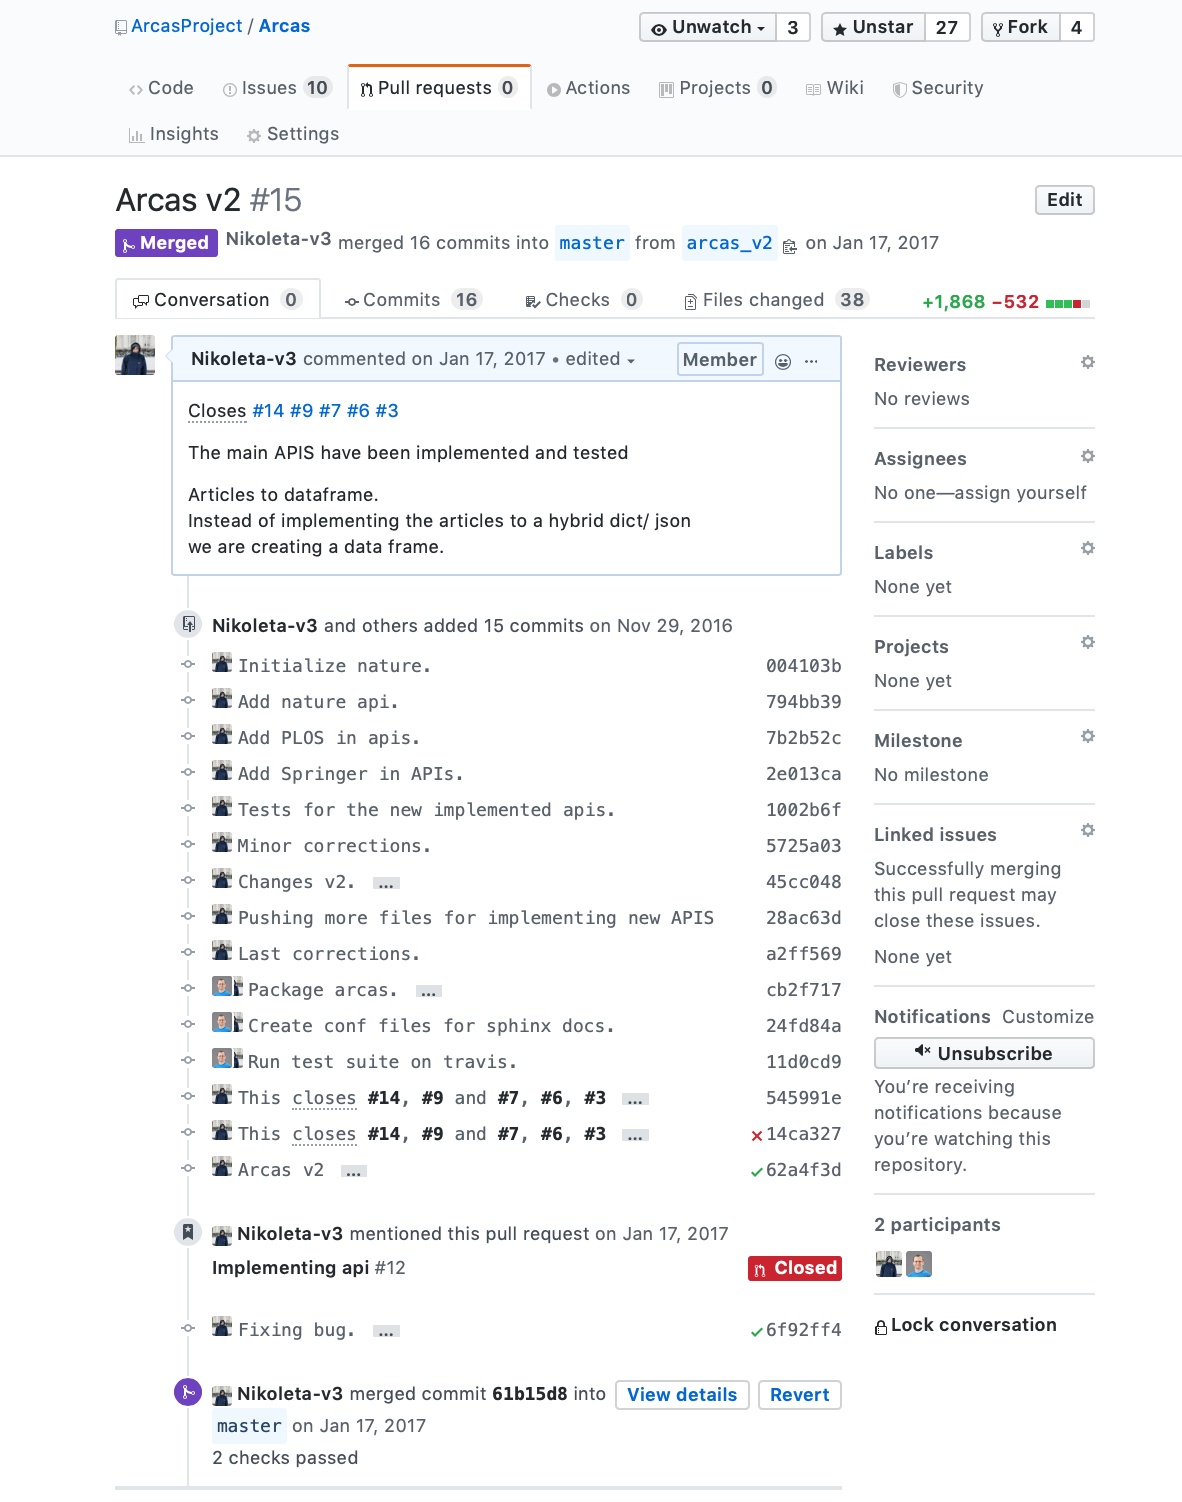
\includegraphics[width=\textwidth]{src/chapters/01/img/GitHub_discussion}
\end{subfigure}
\begin{subfigure}{0.5\textwidth}
    \centering
    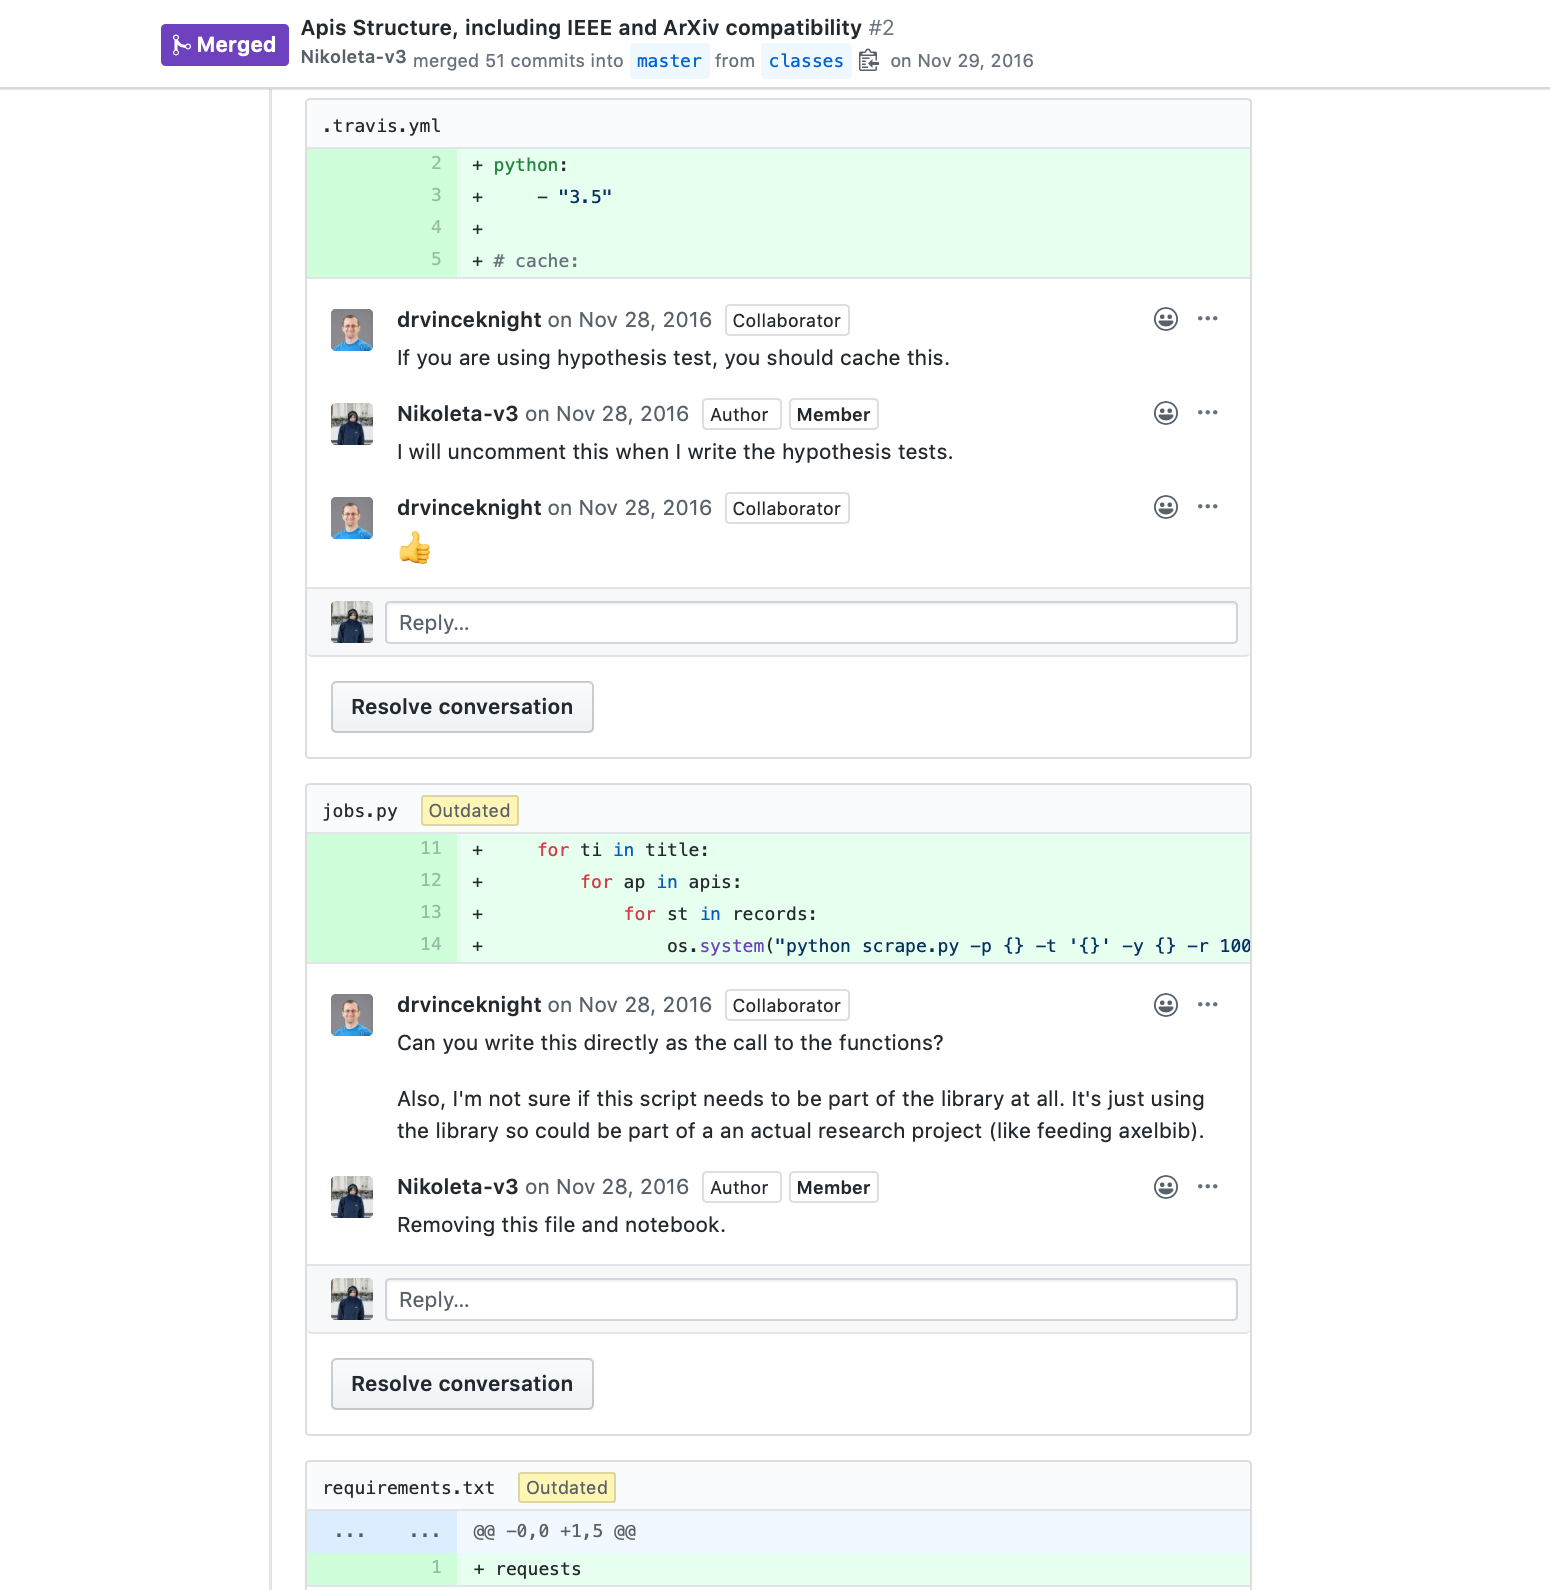
\includegraphics[width=\textwidth]{src/chapters/01/img/GitHub_discussion_two}
\end{subfigure}
\caption{An example of a pull request on GitHub.}\label{fig:pull_request_github}
\end{figure}

The code for Chapters'~\ref{chapter:bibliometric_study}-\ref{chapter:lstm} is
hosted on individual GitHub repositories,
Table~\ref{table:source_code_data_citations}. The source code for each
repository has been packaged and has been archived on Zenodo~\cite{zenodo}.
Zenodo is a platform where code, data and other project elements can be
permanently archived. Zenodo does this by assigning projects a Digital Object
Identifier (DOI) which makes the work citable.

\subsection{Virtual environments}

The source code of each repository has Python libraries as dependencies. Though
several of these projects use the same libraries, the versions of these
libraries can differ. Tracking software dependencies is of paramount importance
in order to ensure the reproducibility of computer code.

There are several tools for keeping dependencies required by different projects
separated. The tool used here are Python \textit{virtual environments}. More
specifically, the Anaconda virtual environments which integrate easily with the
programming language Python. Anaconda~\cite{anaconda} is a free and open-source distribution of
the Python and R programming languages for scientific computing, that aims to
simplify package management and deployment. Package versions are managed by the
package management system conda.

The Anaconda
distribution manager: conda allows users to create, export, list, remove, and update environments that
have different versions of Python and/or packages installed in them. Switching
or moving between environments is called activating the environment. An environment
can be shared and kept under version control as a file. An example of
such as file is given by Figure~\ref{fig:environment_file}.

\begin{figure}[!htbp]
\begin{shell}
name: opt-mo
channels:
  - defaults
dependencies:
  - python=3.6.7
  - numpy=1.15.4
  - pandas=0.23.4
  - pip:
    - attrs==19.1.0
    - axelrod==4.4.0
    - black==18.9b0
    - sympy==1.2.0
    - scikit-optimize==0.5.2
    - jupyter==1.0.0
    - jupyter-console==5.2.0
    - ipython==6.4.0
    - pytest==4.0.1
    - pytest-cov==2.7.1
    - sqlalchemy==1.2.17
    - fsspec==0.3.3
\end{shell}
\caption{An example of an environment file. The name of the specific environment is called
\mintinline{shell}{opt-mo} and it corresponds to the environment associated with
Chapter~\ref{chapter:memory_one}.}\label{fig:environment_file}
\end{figure}

Each Chapter's repository includes an environment file detailing the dependencies
of the source code and their versions.

\subsection{Automated testing}

Testing code is of considerable importance in order to ensure the robustness,
correctness and sustainability of the computer code. The standard method of testing code is through
\textit{automated testing} using test suits that run parts of the code and
assert whether they are behaving as expected.

Two types of tests are described in~\cite{Percival2014}, \textit{functional
tests} that assert the code's functionality, and \textit{unit tests} that help
ensure the code is clean and free of bugs.

Functional tests aim to test how the whole application functions from the
perspective of the outside user. They feed in basic input and test whether the
end product/final behaviour is as expected. Unit tests assert that small chunks
of code behave as expected, and the test the application from the point of the
programmer. Unit tests are isolated from the rest of the code and are modular.
There are two types of unit tests: \textit{pure} and \textit{integrated} tests.

Pure unit tests are written to test only one function or method. Thus, if a pure
unit test was to fail then it should be due to problems with the specific part
of the code it is testing only, and not any other bit of code. Pure unit tests
are fast and readable, however, they do not test how well functions and methods
integrate with one another. This is tested by writing unit tests
that rely on other parts of the code that are not explicitly being tested. This
type of unit test is called integrated tests.

Automated tests, which include functional and unit tests, have been implemented
for the repositories associated with the thesis. This was done using the Python
library \mintinline{python}{pytest} which makes it easy to write automated tests
in a few lines and to check for code coverage. Coverage is a measure used to
describe how much of the code is executed (covered) by the testing suite.
Coverage is tested using a plugin to \mintinline{python}{pytest}, the
\mintinline{python}{pytest-cov}.

To regularly test code which aims to be merged back into the original codebase
continuous integration (CI) systems are used. CIs perform the tests suite and
the coverage checks every time a new version of the codebase is made available
(``pushed'') on GitHub. The benefits of using a CI are identifying bugs quickly,
reducing problems when merging in contributions from collaborators, and adding
transparency to the development process. There are two CIs that have been used
in the repositories listed in Table~\ref{table:source_code_data_citations}.
These are Travis~\cite{travis} and GitHub Actions~\cite{github_actions}.

\subsection{Documentation}

Software \textit{documentation} is written text or illustration that accompanies
computer software or is embedded in the source code. The documentation either
explains how the software operates or how to use it.

Each repository associated with the thesis includes a detailed README file.
These contain installation instructions for the corresponding packaged source code
and demonstrate how to run the associated test suite. The source code for each
repository has been written in a modular way and meaningful names have been
given to all variables, functions, methods and classes. Each function, method
and class includes a \text{docstring}. A docstring is a series of sentences used
to document a specific segment of code.

The repositories also include a series of Jupyter Notebooks~\cite{jupyter} that
are used to carry out the analysis of each Chapter, and serve as demonstration
of the source code's usage.

\subsection{Summary of software written}

As previously stated the codebases for
Chapters~\ref{chapter:bibliometric_study}-\ref{chapter:lstm} have been written
following best practices, have been packaged, are available on GitHub and have
been archived on Zenodo. These practices have been followed to ensure the
correctness, reproducibility and sustainability of the source code and research
described throughout the thesis.

To ensure the reproducibility of the work the data sets used in several of
the following Chapters have also been archived and are available online. The details
for the source code and data sets for each Chapter are summarised in
Table~\ref{table:source_code_data_citations}.

\begin{table}[htbp]
    \centering
    \resizebox{\textwidth}{!}{
    \begin{tabular}{clcc}
        \toprule
        {} & GitHub url & Source code archive & Data archive \\
        \midrule
        Chapter~\ref{chapter:bibliometric_study}    & \url{https://github.com/Nikoleta-v3/bibliometric-study-of-the-prisoners-dilemma} &
        \cite{nikoleta_2017} &  \cite{auction_data_2018, anarchy_data_2018, pd_data_2018} \\
        Chapter~\ref{chapter:meta_tournaments}      & \url{https://github.com/Nikoleta-v3/meta-analysis-of-prisoners-dilemma-tournaments} &
        \cite{Glynatsi_2020_meta_repo} & \cite{Glynatsi2019_meta, Glynatsi2019_meta_raw_data} \\
        Chapter~\ref{chapter:memory_one}            & \url{https://github.com/Nikoleta-v3/Memory-size-in-the-prisoners-dilemma}  &
        \cite{Glynatsi2019_opt_mo} & \cite{glynatsi2019} \\
        Chapter~\ref{chapter:best_response_sequence} \&~\ref{chapter:lstm} & \url{https://github.com/Nikoleta-v3/Training-IPD-strategies-with-RNN} &
        \cite{Glynatsi_2020_sensei} & \cite{Glynatsi2020_sequences, Glynatsi_2020_lstm_weights, Glynatsi_2020_training_data_sets} \\
        \bottomrule
    \end{tabular}}
    \caption{A summary of the GitHub repositories, source code and data archives associated with the thesis.}
    \label{table:source_code_data_citations}
\end{table}

Throughout the thesis, parts of the source code and examples of the code's usage are
going to be presented in the corresponding Chapters. Two types of code snippets
are used in this thesis to present code. Code snippets that demonstrate the
source code of a specific piece of software, Figure~\ref{figure:source_code_example}, and
code snippets that demonstrate the usage,
Figure~\ref{figure:usage_code_example}. These can be distinguish by the three arrows,
\mintinline{python}{>>>}, which are only found in the usage code snippets.
The three arrows are followed by a command. It
demonstrates that the command is executed in a Python interpreter, and the result of executing the command
is the one in the following lines without the arrows.
The code snippets can also be distinguish by their background color. The usage
snippets have a lighter background.

\begin{figure}[htbp]
\begin{sourcepy}
import axelrod as axl

def simulate_match_utility(player, opponent, turns=500, repetitions=200):
    """
    Returns the simulated utility of a memory one player against a single opponent.
    """
    total = 0
    players = [axl.MemoryOnePlayer(vector) for vector in [player, opponent]]
    for rep in range(repetitions):
        match = axl.Match(players=players, turns=turns)
        _ = match.play()

        total += match.final_score_per_turn()[0]

    return total / repetitions
\end{sourcepy}
\caption{Example of a function implemented withing the package
\mintinline{python}{opt_mo} which is the package that has been developed to
carry out the research of Chapter~\ref{chapter:memory_one}.}\label{figure:source_code_example}
\end{figure}

\begin{figure}[htbp]
\begin{usagepy}
>>> import opt_mo
>>> opt_mo.utility.simulate_match_utility([1, 0, 1, 0], [1, 1, 1, 1])
3.0

\end{usagepy}
\caption{An example of using the function \mintinline{python}{simulate_match_utility}
given by Figure~\ref{figure:source_code_example}.}\label{figure:usage_code_example}
\end{figure}

The results of this thesis heavily rely not only on the projects of
Table~\ref{table:source_code_data_citations} but also on the open source package
Axelrod-Python library (APL). APL~\cite{axelrodproject} is an open source
project for simulating rounds of the IPD which contains a large collections of
strategies. APL has several capabilities which include performing different
types of tournaments. Its documentation is found at
\url{http://axelrod.readthedocs.io/}. The specific version of APL used in each
Chapter will be mentioned at the start of each Chapter.

This thesis itself is hosted on a GitHub repository at
\url{https://github.com/Nikoleta-v3/Thesis}. It is written in the document
preparation system \LaTeX, and automated tests have been setup to test
that the document compiles, spelling is correct, every time
an updated version of the document is pushed to GitHub. The usage code examples
of this thesis are also automatically tested. Each command beginning with the
symbol \mintinline{python}{>>>} is executed each time the document is pushed to GitHub.
The test executes the commands and checks that the outcome is the
same as the one following the command in the code snippets.

\section{Chapter summary}

This Chapter has introduced the IPD which is the
strategic game used in this thesis. It has presented a review of the Axelrod's
tournaments in the 1980s, and presented a list of tournaments that have been
performed ever since.

The research questions of this thesis and how each Chapter contributes to these
questions have been outlined. The research of this thesis heavily reliefs on
software. The software includes already established packages and packages that
have been developed specifically for this thesis. These have been developed
following best practices. A number of best practices were introduced in
section~\ref{section:introduction_software_development}.

The software packages and the data sets used in the following Chapters have been
archived and made available online. This reassures that all the results
presented in the following Chapters are reproducible. The developed packages as
well as this thesis are being hosted on GitHub repositories and are being tested
using automated tests.
